\section{Evietania Charis Sujadi}
\subsection{Fungsi Csv}
Fungsi csv yaitu memudahkan user dalam melakukan input data karena pada csv input data ataupun import data dalam skala besar dapat dilakukan dengan cara yang sederhana.
\subsection{Sejarah Csv}
Dari rilis pertama, Excel menggunakan format file biner yang disebut Binary Interchange File Format (BIFF) sebagai format file utamanya. Ini berubah ketika Microsoft merilis Office System 2007 yang memperkenalkan Office Open XML sebagai format file utamanya. Office Open XML adalah file kontainer berbasis XML yang mirip dengan XML Spreadsheets (XMLSS), yang diperkenalkan di Excel 2002. File versi XML tidak bisa menyimpan makro VBA. Meskipun mendukung format XML baru, Excel 2007 masih mendukung format lama yang masih berbasis BIFF tradisional. Selain itu Microsoft Excel juga mendukung format Comma Separated Values (CSV), DBase File (DBF), SYMbolic LinK (SYLK), Format Interchange Data (DIF) dan banyak format lainnya, termasuk format lembar kerja 1-2 Lotus - 3 (WKS, WK1, WK2, dll.) Dan Quattro Pro.
\lstinputlisting[firstline=7, lastline=20]{src/4/1174051/teori/gatau.py}
\subsection{Aplikasi yang dapat menghasilkan csv}
\begin{itemize}
\item Texteditor
Seperti notepad++,visual studio code,atom,sublime dan lain sebagainya
\item Program Spreadsheet
  Seperti excell,google spreadshare,LibreOfficecalc
 \end{itemize}
\subsection{Jelaskan bagaimana cara menulis dan membaca file csv di excel atau spreadsheet}
Caranya sangat mudah yaitu:
 Untuk menulisnya untuk yang paling atas itu kita buat headernya,untuk mepermudah membedakan datanya,dan untuk baris kedua dan seterusnya itu untuk data itu sendiri.Setelah di buat kalian save as kemudian pilih format CSV.Untuk membukan cukup di double clik file tersebut
\subsection{Jelaskan sejarah library csv}
CSV muncul untuk memudahkan data science dan analis karena dinilai terdapat banyak kemudahan yang didapat. CSV dapat dimaksimalkan jika dipaduka dengan python karena python adalah bahasa pemrograman yang support ke banyak library termasuk csv. Maka karena itulah perpaduan python dan csv seringkali digunakan oleh perusahaan-perushaan besar dalam mengolah datanya.
\subsection{Jelaskan sejarah library pandas}
Pandas merupakan tool yang dapat digunakan sebagai alat analisis data dan struktur untuk bahasa pemrograman Python. Pandas dapat mengolah data dengan mudah, salah satu fitur yang ada dalam pandas adalah Dataframe. Fitur dataframe dapat membaca sebuah file dan menjadikannya tabble, juga dapat mengolah suatu data dengan menggunakan operasi seperti join, group by dan teknik lainnya yang terdapat pada SQL. Dalam hal ini pandas tidak jauh beda dengan csv yaitu memiliki keunggulan dalam pengolahan data-data besar dan dapat disupport dengan baik dengan python walaupun mengimport data dalam jumlah banyak.
\subsection{Fungsi-fungsi Library CSV}
Dalam library csv terdapat dua fungsi yaiut fungsi membaca file dan menulis file csv.
Library csv mempunyai keunggulan dibandingkan format data lainnya adalah soal kompatibilitas. File csv dapat digunakan, diolah, diekspor/impor, dan dimodifikasi menggunakan berbagai macam perangkat lunak dan bahasa pemrograman. Pada library csv mempunyai fungsi import dan eksport data yang baik dan bisa digunakan dalam jumlah besar.
\subsection{Fungsi-fungsi library Pandas}
Pandas pun memiliki fungsi yang sama yaitu menulis dan membaca file. pandas menyediakan beragam fungsi operasi untuk mengolah data. Contoh jika menggunakan series bisa mencari nilai max, min, dan mean secara langsung, bahkan juga bisa melakukan operasi perpangkatan pada nilai Series secara langsung.
Pandas dapat mengolah suatu data dan mengolahnya seperti join, distinct, group by, agregasi, dan teknik seperti pada SQL. Hanya saja dilakukan pada tabel yang dimuat dari file ke RAM.
\subsection{Bukti Plagiarisme}
\begin{figure}[h]
	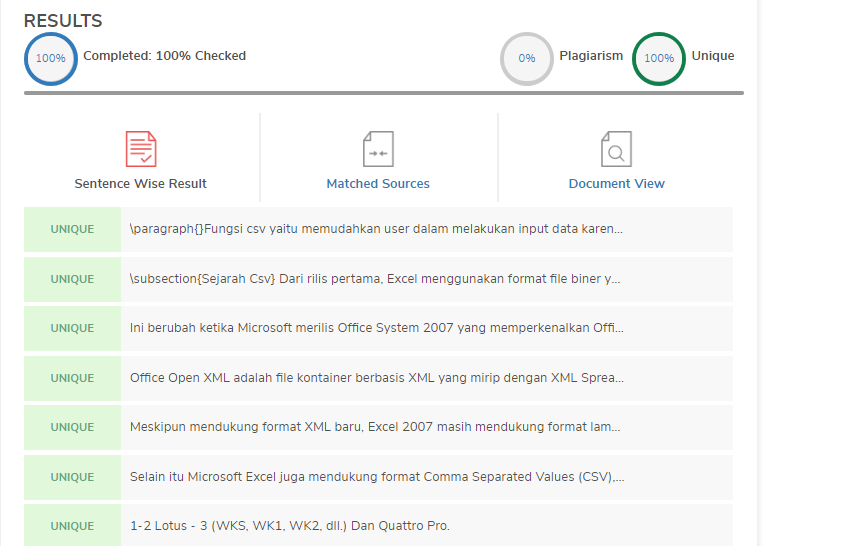
\includegraphics[width=10cm]{figures/4/1174051/teori/nih.png}
	\centering
\end{figure}
\section{Muhammad Dzihan Al-Banna}
\subsection{Soal 1}
Comma Separated Value atau CSV adalah format data yang memudahkan penggunanya melakukan input data ke database secara sederhana. CSV dapat digunakan dalam standar file ASCII. Dalam format csv record dipisahkan dengan tanda koma atau titik koma. Ketika user menerima file dengan format CSV, yang biasanya bertuliskan .CSV, maka file tersebut akan terbuka dalam format Microsoft Excel. CSV muncul demi memenuhi kebutuhan perusahaan-perusahaan besar dalam mengolah data yang banyak.
\lstinputlisting[firstline=7, lastline=20]{src/4/1174095/cobacsv.py}
\subsubsection{Fungsi}
Fungsi csv yaitu memudahkan user dalam melakukan input data karena di csv input data atau import data dalam skala besar dapat dilakukan dengan cara yang sederhana.
\subsection{Soal 2}
Ada beberapa aplikasi yang dapat menghasilkan file dengan format csv diantaranya google sheet, number di MacOS dan microsoft excel.
\subsection{Soal 3}
cara membuat file csv di excel cukup mudah yaitu :
\begin{itemize}
	\item Buat foldernya
	\item Pilih save as
	\item pilih file dengan format csv
\end{itemize}
cara membaca file di csv :
\begin{itemize}
	\item Klik data get external data form text
	\item Akan muncul Text Import Wizard, arahkan pada file csv yang ingin anda buka Open.
	\item Setelah File terbuka, akan muncul Text Import Wizard.
	\item Pilih Delimited, Kemudian Next (Di sini, bisa juga menentukan baris awal yang akan di import)
	\item Centrang pada Tab dan Comma (Atau sesuai pengaturan File Anda) Next.
	\item Atur Format data pada tiap kolom yang tampil dan klik Finish
\end{itemize}
\subsection{Soal 4}
CSV muncul untuk memudahkan data science dan analis karena dinilai terdapat banyak kemudahan yang didapat. CSV dapat dimaksimalkan jika dipaduka dengan python karena python adalah bahasa pemrograman yang support ke banyak library termasuk csv. Maka karena itulah perpaduan python dan csv seringkali digunakan oleh perusahaan-perushaan besar dalam mengolah datanya.
\subsection{Soal 5}
Pandas merupakan tool yang dapat digunakan sebagai alat analisis data dan struktur untuk bahasa pemrograman Python. Pandas dapat mengolah data dengan mudah, salah satu fitur yang ada dalam pandas adalah Dataframe. Fitur dataframe dapat membaca sebuah file dan menjadikannya tabble, juga dapat mengolah suatu data dengan menggunakan operasi seperti join, group by dan teknik lainnya yang terdapat pada SQL. Dalam hal ini pandas tidak jauh beda dengan csv yaitu memiliki keunggulan dalam pengolahan data-data besar dan dapat disupport dengan baik dengan python walaupun mengimport data dalam jumlah banyak.
\subsection{Soal 6}
Dalam library csv terdapat dua fungsi yaiut fungsi membaca file dan menulis file csv.
Library csv mempunyai keunggulan dibandingkan format data lainnya adalah soal kompatibilitas. File csv dapat digunakan, diolah, diekspor/impor, dan dimodifikasi menggunakan berbagai macam perangkat lunak dan bahasa pemrograman. Pada library csv mempunyai fungsi import dan eksport data yang baik dan bisa digunakan dalam jumlah besar.
\subsection{Soal 7}
Pandas pun memiliki fungsi yang sama yaitu menulis dan membaca file. pandas menyediakan beragam fungsi operasi untuk mengolah data. Contoh jika menggunakan series bisa mencari nilai max, min, dan mean secara langsung, bahkan juga bisa melakukan operasi perpangkatan pada nilai Series secara langsung.
Pandas dapat mengolah suatu data dan mengolahnya seperti join, distinct, group by, agregasi, dan teknik seperti pada SQL. Hanya saja dilakukan pada tabel yang dimuat dari file ke RAM.
\subsection{Bukti Plagiarisme}
\begin{figure}[h]
	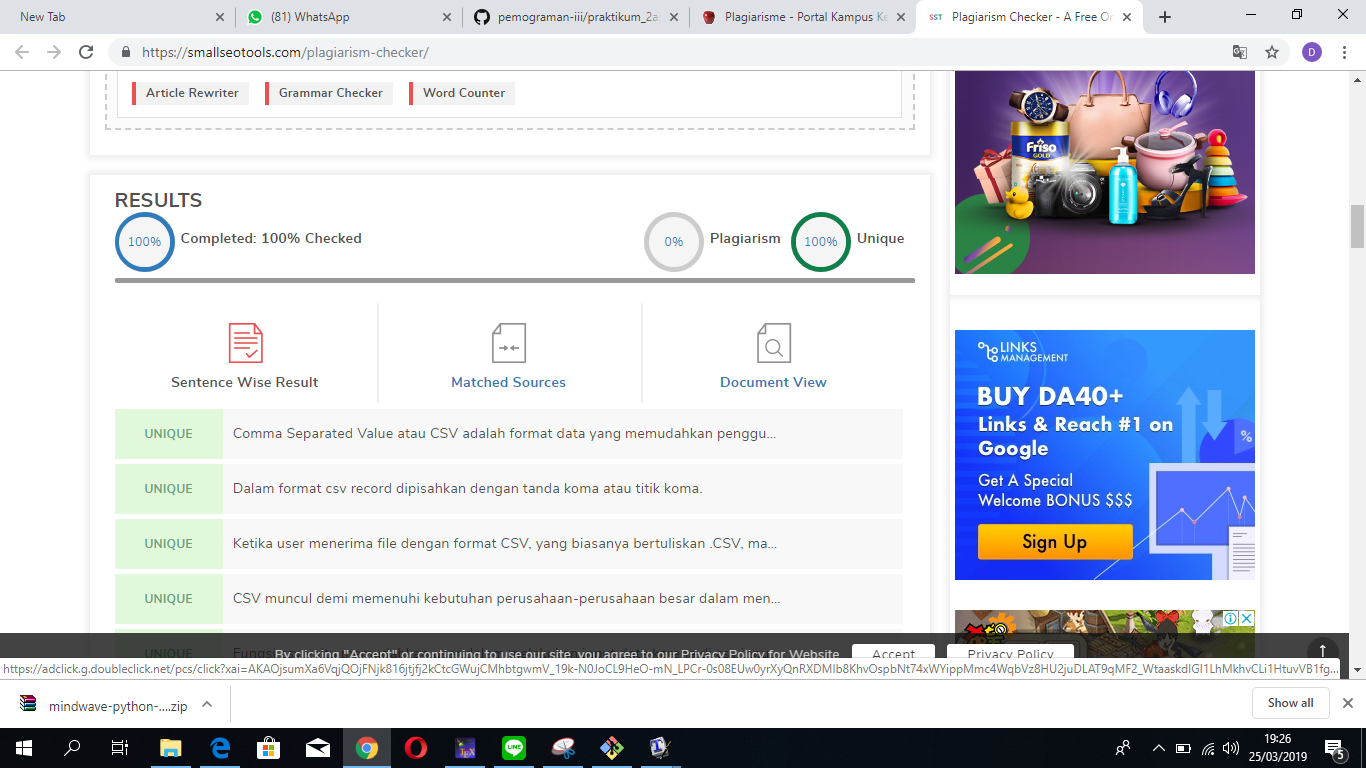
\includegraphics[width=10cm]{figures/4/1174095/bukti.png}
	\centering
\end{figure}

\section{Nico Ekklesia Sembiring}
\subsection{Apa itu fungsi file csv, jelaskan sejarah dan contoh.}
File CSV(Comma Separated Value) merupakan format data yang dapat memudahkan pengguna ketika akan melakukan input data kedalam database sederhana. Pada penggunaan CSV, setiap record dipisahkan dengan koma atau titik koma.

	Sejarah CSV adalah  dimulai pada tahun 1972, dimana pada saat itu digunakan pada IBM Fortran dibawah dukungan OS / 360. pada saat itu input/output diarahkan kepada Fortran77 hingga akhirnya disetujui pada tahun 1978. CSV mulai digunakan oleh pada tahun 1983. Inisiatif standardisasi utama - mentransformasikan "definisi fuzzy de facto" menjadi definisi yang lebih tepat dan de jure - adalah pada tahun 2005, dengan RFC4180, mendefinisikan CSV sebagai Tipe Konten MIME. Kemudian, pada 2013, beberapa kekurangan RFC4180 ditangani oleh rekomendasi W3C. Pada 2014 IETF menerbitkan RFC7111 yang menjelaskan aplikasi fragmen URI pada dokumen CSV. RFC7111 menentukan bagaimana rentang baris, kolom, dan sel dapat dipilih dari dokumen CSV menggunakan indeks posisi. Pada 2015 W3C, dalam upaya untuk meningkatkan CSV dengan semantik formal, mempublikasikan draft rekomendasi pertama untuk standar metadata CSV, yang dimulai sebagai rekomendasi pada bulan Desember tahun yang sama.
contohnya adalah :
\lstinputlisting[firstline=2, lastline=5]{src/4/1174096/teori/1174096.csv}

\subsection{Aplikasi-aplikasi apa saja yang bisa menciptakan file csv?}
Aplikasi yang dapat menciptakan file CSV terdiri dari Text Editor seperti Notepad, Notepad, Sublime, Visual Studio Code. Aplikasi lainya yang dapat digunakan Microsoft Excel, Google Spreadsheet, LibreOffice Calc.

\subsection{Jelaskan bagaimana cara menulis dan membaca file csv di excel atau spreadsheet.}
Cara menulis File CSV di Excel adalah sebagai berikut :
	\begin{itemize}
	\item Download terlebih dahulu template csv
	\item Setelah itu buka Google Sheet di Browser
	\item Buat spreadsheet baru dengan mengklik tanda + yang berada di pojok kanan bawah
	\item Pilih menu File, kemudian pilih open
	\item Setelah Pilihan open terbuka, lalu pilih tab Upload. setelah itu klik pada tombol Pilih File dari perangkat anda
	\item Cari dan buka file template yang telah di download sebelumnya
	\item Setelah ini pengguna dapat menambahkan data pada kolom maupun baris sesuai dengan keinginan pengguna
	\item Setelah selesai mengedit, sekarang pengguna harus melakukan eksport file ke file csv.
	\end{itemize}

Sedangkan cara membaca file CSV dengan excel adalah sebagai berikut :
	\begin{itemize}
	\item Pertama-tama yang dilakukkan adalah membuka Ms. Excel
	\item pilih menu DATA, lalu pilih from text, pilih File CSV, lalu OK
	\item Akan muncul kutak Text Iport Wizard yang nantinya muncul data file csv yang ingin diimport
	\item pada delimiters, pilih menu comma, kemudian pilih Next
	\item pada kolom format pilih general jika terdapat text maupun tanggal. Lalu pilih Finish
	\item Selanjutnya akan muncul kotak import data. Pilih pada Existing Worksheet, lalu pilih OK.
	\end{itemize}

\subsection{Jelaskan sejarah library csv}
Library csv pada awalnya dibuat untuk memperudah dalam melakukan pengolahan data. Dan mempermudah untuk melakukan export dan import file csv itu sendiri

\subsection{Jelaskan sejarah library pandas}
Sejarah Pandas dimulai dari Pengembang Wes McKinney yang mulai mengerjakan pandas pada 2008 pada saat berada di AQR Capital Management dikarenakan kebutuhan akan alat kinerja tinggi yang fleksibel untuk melakukan analisis kuantitatif pada data keuangan. Sebelum meninggalkan AQR, dia bisa meyakinkan manajemen untuk mengizinkannya membuka sumber perpustakaan.

Pegawai AQR lainnya, Chang She, bergabung dengan upaya ini pada 2012 sebagai kontributor utama kedua ke perpustakaan.

Pada 2015, pandas menandatangani sebagai proyek NumFOCUS yang disponsori secara fiskal, sebuah badan amal nirlaba 501 (c) (3) di Amerika Serikat.

\subsection{Jelaskan fungsi-fungsi yang terdapat di library csv}
Fungsi dalam library CSV terbagi menjadi beberapa bagian. yaitu:
	\begin{itemize}
	\item fungsi membaca file csv.
    	fungsi ini bisa dipanggil dengan list dan dictionary
    	Dengan list :
    	\lstinputlisting[firstline=11, lastline=21]{src/4/1174096/teori/1174096.py}
    	Dengan dictionary :
    	\lstinputlisting[firstline=24, lastline=33]{src/4/1174096/teori/1174096.py}
   	 \item fungsi menulis file csv.
    	\lstinputlisting[firstline=36, lastline=40]{src/4/1174096/teori/1174096.py}
	\end{itemize}

\subsection{Jelaskan fungsi-fungsi yang terdapat di library pandas}
Fungsi- fungsi yang terdapat di library pandas hampir sama dengan fungsi pada library csv,akan tetapi pada library pandas penulisannya lebih sederhana dari pada library csv sehingga terlihat lebih rapi.
		\lstinputlisting[firstline=43, lastline=44]{src/4/1174096/teori/1174096.py}
\subsection{Cek Plagiarisme}
	\begin{figure}[!htbp]
	\centering
	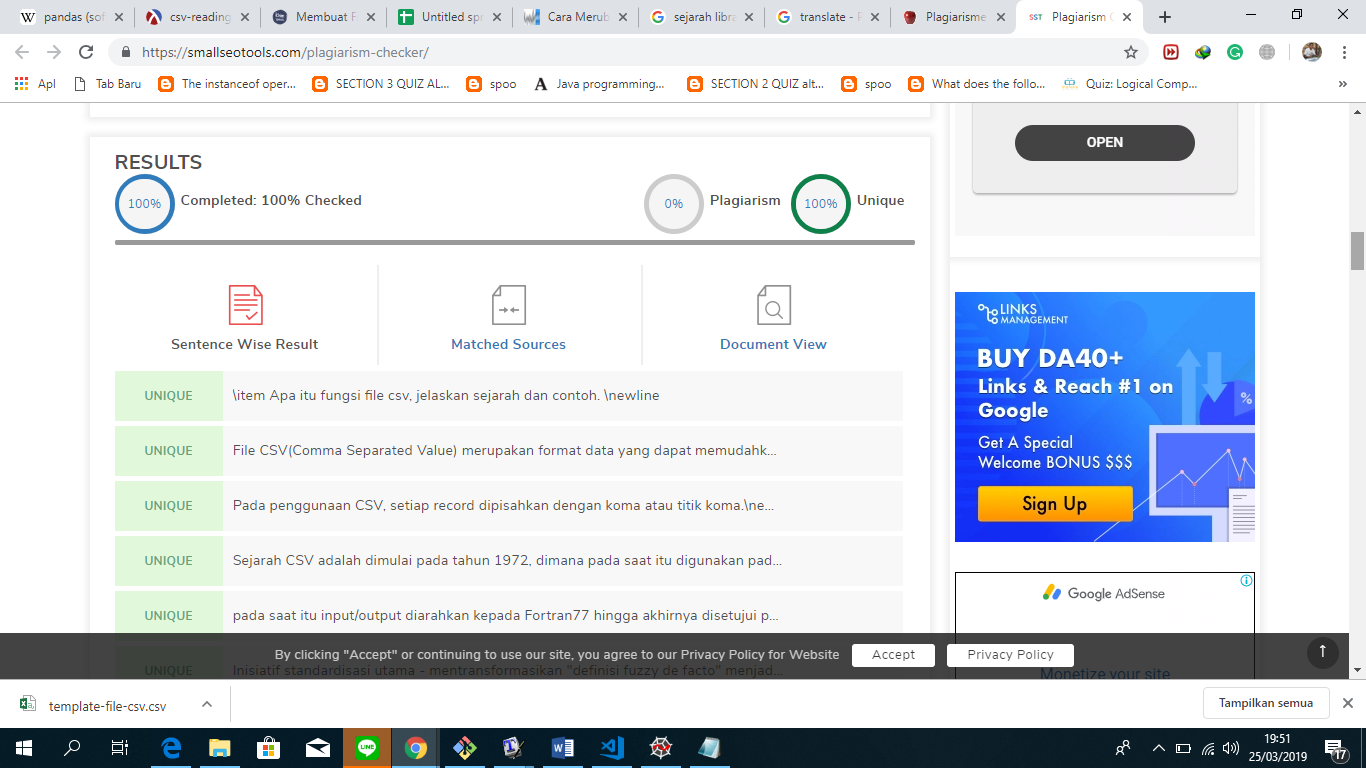
\includegraphics[width=9cm,height=6cm]{figures/4/1174096/teori/plagiarisme.png}
	\caption{Plagiarisme}
	\label{plagiarisme}
	\end{figure}

\section{Oniwaldus Bere mali}
\subsection{Teori}
\section{Oniwaldus Bere Mali}
\begin{enumerate}
\item Fungsi file csv,sejarah dan contoh :
File CSV (Comma Limited Value) adalah jenis file khusus yang dapat Anda buat atau edit di Excel. File CSV menyimpan informasi yang dipisahkan oleh koma, tidak menyimpan informasi dalam kolom. Ketika teks dan angka disimpan dalam file CSV, mudah untuk memindahkannya dari satu program ke program lainnya.
Dari rilis pertama, Excel menggunakan format file biner yang disebut Binary Interchange File Format (BIFF) sebagai format file utamanya. Ini berubah ketika Microsoft merilis Office System 2007 yang memperkenalkan Office Open XML sebagai format file utamanya. Office Open XML adalah file kontainer berbasis XML yang mirip dengan XML Spreadsheets (XMLSS), yang diperkenalkan di Excel 2002. File versi XML tidak bisa menyimpan makro VBA.
Meskipun mendukung format XML baru, Excel 2007 masih mendukung format lama yang masih berbasis BIFF tradisional. Selain itu Microsoft Excel juga mendukung format Comma Separated Values (CSV), DBase File (DBF), SYMbolic LinK (SYLK), Format Interchange Data (DIF) dan banyak format lainnya, termasuk format lembar kerja 1-2 Lotus - 3 (WKS, WK1, WK2, dll.) Dan Quattro Pro.
\item Aplikasi yang bisa menciptakan file csv :
\begin{itemize}
\item Texteditor
Seperti notepad++,visual studio code,atom,sublime,notepad dan lain sebagainya
\end{itemize}
\item Cara menulis dan membaca file csv di excel atau spreadsheet :
Untuk menulisnya untuk yang paling atas itu kita buat headernya,untuk mepermudah membedakan datanya,dan untuk baris kedua dan seterusnya itu untuk data itu sendiri.
dan setelah di buat kalian save as kemudian pilih format CSV.
dan untuk membukan cukup di double clik file tersebut
\item Sejarah library csv:
library csv dibuat untuk permudah mengolah data. Dan mempermudah untuk melakukan export dan import file csv itu sendiri
\item Sejarah library pandas dari :
library pandas dibuat agar bahasa pemograman python bisa bersaing R dan matlab, yang digunakan untuk mengolah banyak data , keperluan big data, data mining data science dan sebagainya.
\item Fungsi-fungsi yang terdapat di library csv :
Dalam librarycsv terdapat 2 fungsi yang bisa digunakan oleh library csv
Pertama,fungsi membaca file csv.
fungsi ini bisa menggunakan list dan dictionarys
\item Fungsi-fungsi yang terdapat di library pandas :
Hampir sama dengan library csv,tp library pandas penulisannya lebih sederhana dan terlihat lebih rapih dari pada library csv.
\end{enumerate}
\subsection{Cek Plagiarisme}
\begin{figure}[!htbp]
\centering
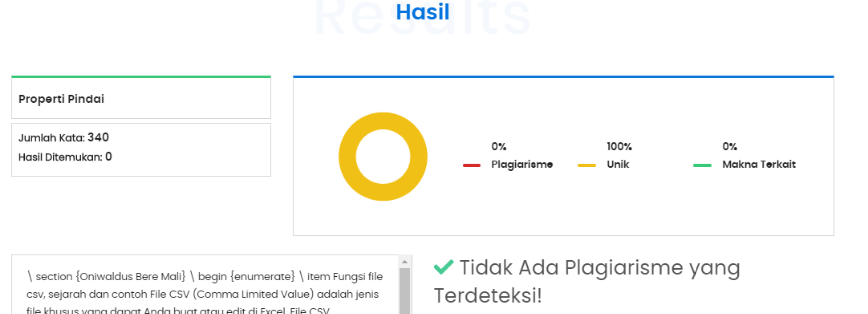
\includegraphics[width=3cm,height=3cm]{figures/4/1174005/plagiat.PNG}
\caption{Plagiarisme}
\label{plagiarisme}\end{figure}




Kalau mau dibikin paragrap \textbf{cukup enter aja}, tidak usah pakai \verb|par| dsb

%\subsection{Soal 2}
%Isi jawaban soal ke-2

%\subsection{Soal 3}
%Isi jawaban soal ke-3

\section{Doli Jonviter}
\subsection{Soal 1}
Isi jawaban soal ke-1

Kalau mau dibikin paragrap \textbf{cukup enter aja}, tidak usah pakai \verb|par| dsb

%\subsection{Soal 2}
%Isi jawaban soal ke-2

%\subsection{Soal 3}
%Isi jawaban soal ke-3

\section{Rahmatul Ridha}
\subsection{Soal 1}
Isi jawaban soal ke-1

Kalau mau dibikin paragrap \textbf{cukup enter aja}, tidak usah pakai \verb|par| dsb

%\subsection{Soal 2}
%Isi jawaban soal ke-2

%\subsection{Soal 3}
%Isi jawaban soal ke-3

\section{Tomy Prawoto}
\subsection{Soal 1}
Isi jawaban soal ke-1

Kalau mau dibikin paragrap \textbf{cukup enter aja}, tidak usah pakai \verb|par| dsb

%\subsection{Soal 2}
%Isi jawaban soal ke-2

%\subsection{Soal 3}
%Isi jawaban soal ke-3
